\documentclass{JAC2003}
% IPAC 2012 - General document layout
\usepackage[utf8]{inputenc}
\usepackage{graphicx, subfigure,amsmath}
\usepackage{booktabs}


\begin{document}
\title{EVALUATION OF THE BEAM COUPLING IMPEDANCE OF NEW BEAM SCREEN DESIGNS FOR THE LHC INJECTION KICKER MAGNETS}
\author{H. Day\thanks{hugo.day@hep.manchester.ac.uk}$^{\dagger\ddagger\star}$, M.J. Barnes$^{\dagger}$, F. Caspers$^{\dagger}$, R.M. Jones$^{\ddagger \star}$, E. Métral$^{\dagger}$, B. Salvant$^{\dagger}$ \\
$\dagger$ CERN, Switzerland,
$\ddagger$ School of Physics and Astronomy, The University of Manchester, Manchester, UK,\\
$\star$ Cockcroft Institute, Daresbury, UK 
}

\maketitle 


\begin{abstract}
The LHC injection kicker magnets (MKIs) have experienced a significant degree of beam induced heating since the beginning of 2011 due to the increasing intensity stored in the LHC, for long periods of time, and the relatively large broadband beam coupling impedance of the installed kicker magnets. In this paper we show the sources of impedance in the MKIs, and the effect that the beam screen dimensions have on the impedance. We show how these alter the power loss, and present an improved beam screen design that improves shielding on the magnet, whilst further improving the electrical breakdown situation.
\end{abstract}

%Title format - Title; Authors; Affiliation; conference
%Abstract - Copied from submitted abstract (maybe changed to represent changes in presented paper)
%Introduction
%Body of data
%Conclusion
%Acknowledgements
%References

% Aim of paper - To present the causes of the beam coupling impedance in the beam screen - length of overlap, thickness, screening by conductors. Expected power loss for the new screen design with present and HL-LHC parameters
% Sections:
% Introduction - Brief history of the MKI heating - reference to Mike's paper last year and this year
% Reasons for the impedance - Distinction between well screened and not well screened
% - Increasing number of screen conductors reduces effect of the ferrite
% - Dimensions of the capacitive end changing impedance profile
% - Effect of different ferrites on the 30-40MHz peak if time
% Power loss expectactions for HL-LHC, post LS1 between 15, 19 and New design
%
%
%

% Images to include
% New screen design cross section
% New screen design impedance
% Various lengths of overlap impedance and predicted resonant frequency
% 

\section{INTRODUCTION}

During the 2011 and 2012 runs of the LHC, high temperatures were observed in several devices in the LHC  \cite{metral_cham2012}, a critical piece being the LHC injection kicker magnets (MKIs, Fig.~\ref{fig:mkiStruct}), which were attributed to beam-induced heating due to high power loss from the interaction of the circulating beam with the longitudinal beam coupling impedance. This heating was observed to raise the temperature of the ferrite yoke of one of the MKIs above its Curie point during fills, thereby necessitating waiting times of several hours for the ferrite to cool before safe injection could be carried out \cite{mki-heating}. 

In response to this an extensive study to reduce the temperature of the ferrite yoke was carried out, aimed at reducing the power loss into the kicker magnet and increasing the transfer of thermal energy from the ferrite yoke to the surroundings \cite{mki-heatingTemp}. A new beam screen was implemented in MKI8D in technical stop 3 (TS3) (23/09/12-27/09/12) with improved screening of the ferrite from the beam and some modifications to reduce the likelihood of electrical breakdown during magnet pulsing: this was observed to greatly reduce the temperature of the ferrite yoke \cite{mki-heatingTemp}. Building on this success, further modifications to the beam screen have been proposed to further reduce the beam coupling impedance. In addition, the reasons for the resulting impedance in a well screened magnet (i.e. where the beam does not see the ferrite yoke) are discussed. 

\begin{figure}
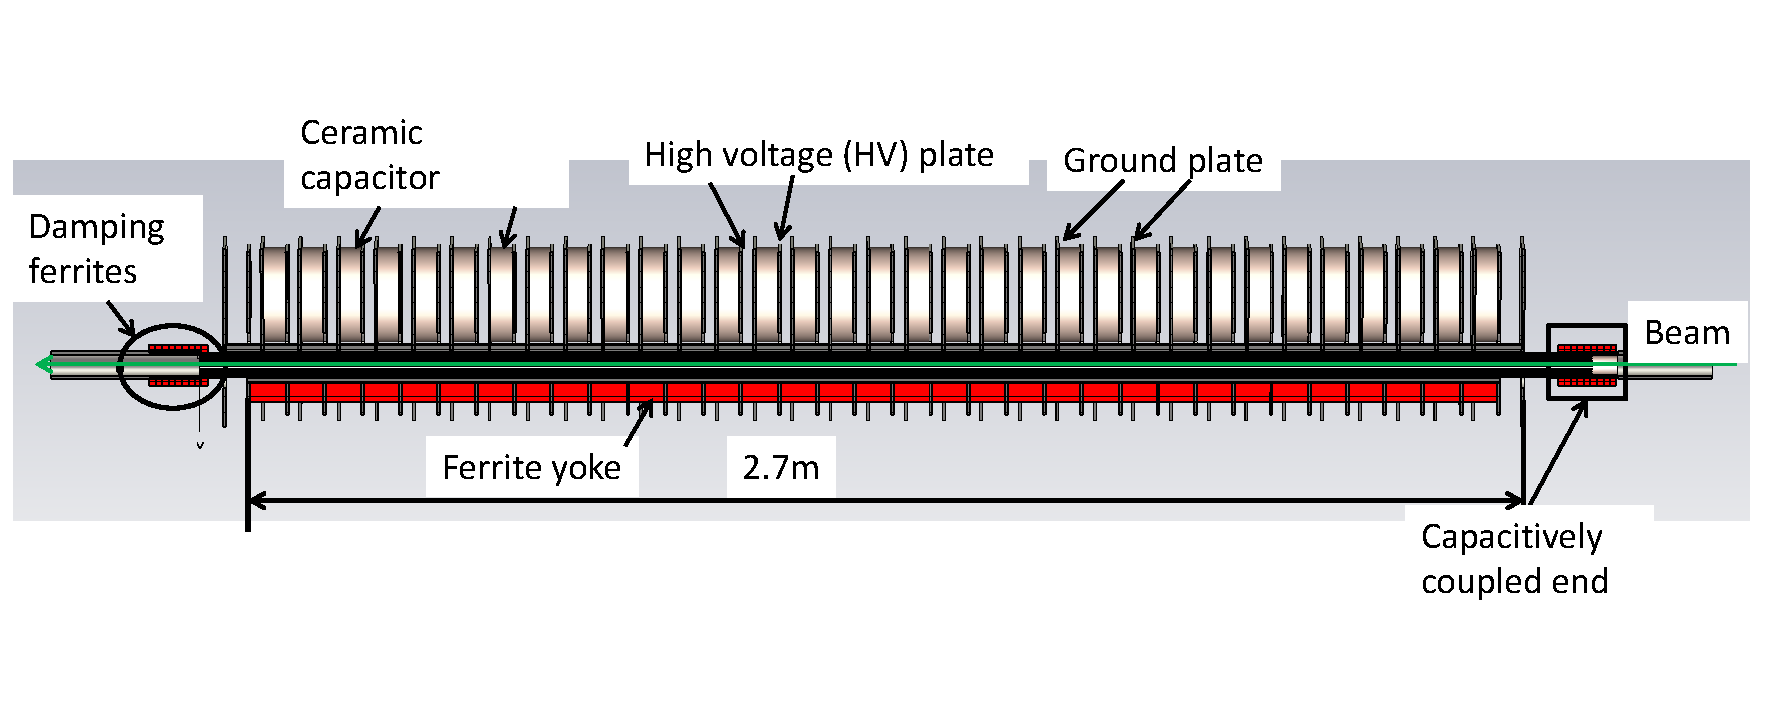
\includegraphics[width=0.5\textwidth]{MKICrossSectionYZ.pdf}
\caption{Structure of the injection kicker magnets.}
\label{fig:mkiStruct}
\end{figure}

\section{NEW BEAM SCREEN DESIGN}

The large real component of the longitudinal impedance of the MKIs as installed in the LHC, during operation during 2011 and 2012, is due to the ferrite still being visible to the circulating beam \cite{kicker_meas}. As such to reduce the power loss in the kickers, it is necessary to improve the screening of the ferrite. This is best achieved by ensuring that all 24 screen conductors are placed into the beam screen of the kicker magnet. The original beam screen design had 24 screen conductors in place, but 9 were removed to decrease flashover on the surface of the capacitively coupled end of the ceramic tube \cite{mki-ElecBreakdown}. 

To this effect many new beam screen designs have been considered to reduce the likelihood of electrical breakdown during pulsing, leading to the design shown in Fig.~\ref{fig:newScreenDesign}. This design greatly reduces the electric field on the capactively coupled end of the screen conductors by stepping the external conductive material away from the surface of the ceramic tube. This allows 24 conductors to be inserted, greatly reducing the beam coupling impedance compared to the impedance of most present MKIs, and compared to the replacement MKI8D installed in TS3 (Fig.~\ref{fig:MKIScreenImp}). The beam coupling impedance simulations were done using a simplified model of the MKI in CST Particle Studio \cite{cst-cite}, using the model represented in Fig.~\ref{fig:mkiStruct}, with a time domain solver: the impedance is subsequently obtained by an FFT of the resulting wakefunction. 

Of particular interest is the change in the nature of the beam coupling impedance; from the broadband impedance characteristic of interactions due to a materials properties that is seen in the case of the kicker magnet with only 15 screen conductors, to a mixed impedance with 19 screen conductors, to a strongly resonant-type impedance in the beam screen with 24 screen conductors. The effort to understand the source of these resonances is also useful to determine whether the beam coupling impedance can be further optimised to reduce heating for any future upgrades of the LHC (to higher bunch intensities or numbers of circulating bunches).

\begin{figure}
\includegraphics[width=0.5\textwidth]{mki-final-design.pdf}
\caption{The proposed beam screen design for the MKI post-LS1.}
\label{fig:newScreenDesign}
\end{figure}

\begin{figure}
\begin{center}\includegraphics[width=0.4\textwidth]{realImp.pdf}
\caption{The real component of the longitudinal beam coupling impedance of the existing MKIs, the replacement MKI8D and the proposed beam screen design for after LS1.}
\label{fig:MKIScreenImp}
\end{center}
\end{figure}

\section{CAUSES OF THE IMPEDANCE}

By placing field monitors in the simulation model it is possible to observe the field patterns of the wakefield. For the MKI beam screen with 24 screen conductors, the strong fields after the beam has traversed an MKI were localised in the region between the screen conductors and the external metallization/metal tube, as seen in Fig.~\ref{fig:mkiResFieldPat}. These are $n \lambda /2$ resonances, where $\lambda$ is the wavelength of the resonance and $n$ an integer. This gave a predicted resonant frequency $f_{res}$ of 

\begin{equation}
f_{res} = \frac{nc}{\sqrt{\epsilon_{r}}2 \left( L_{overlap} + \delta_{fringe} \right)},
\label{eqn:imp-overlap-fres}
\end{equation}

where $\epsilon_{r}$ is the relative permittivity of the surrounding medium (in this case $\epsilon_{r} \approx 10$ for the alumina ceramic tube), $c$ is the speed of light, $L_{overlap}$ is the length of the overlap between the screen conductors and the external metallization/metal tube, and $\delta_{fringe}$ is a factor to take into account fringe fields, which depends on the distance between the screen conductors and the external metallization/metal tube. To illustrate this, a shortened end section of the beam screen with 24 screen conductors has been simulated with a variety of different lengths of overlap (achieved by changing the length of the external metallization), between 80 mm and 120 mm in 10 mm increments. The resulting simulated impedances and predicted resonant frequencies are shown in Fig.~\ref{fig:mkiOverlapRes}, showing very good agreement between the simulated values and the predictions. It has been found that the value of $\delta_{fringe}$ can be estimated from the thickness of the ceramic tube, such that

\begin{equation}
\delta_{fringe} \approx 1.25 \times t_{pipe}
\end{equation}

where $t_{pipe}$ is the ceramic tube thickness in mm. Further effects of the beam screen layout have been examined e.g. the ceramic tube thickness, the number of screen conductors and their orientation: these are presented in depth in~\cite{DayThesis}. Studies on determining the peak height of the resonant impedance are ongoing. 

During 2012 there has been unexpected heating of some toroidal ferrites, nine of which are mounted at each of the ceramic tube in order to damp low-frequency ($<$50 MHz) resonances. One set of toroids, at the capacitively coupled end of the beam screen, occasionally reached 193$^{\circ}$C measured; all others remained below 100$^{\circ}$C measured. The source of this heating is being studied; possible hypotheses are that this may be due to coupling to the resonance due to the overlap of the screen conductors and external metallization/external tube or that the resonant frequency changes due to thermal expansion of the screen conductors. It is planned to carry out detailed measurements to analyse this with the new beam screen in the laboratory.

\begin{figure}
\includegraphics[width=0.5\textwidth]{resField.jpeg}
\caption{A freezeframe of the wakefield of the MKI beam screen with 24 screen conductors. The field can be seen to be localised in the region between the screen conductors and external metallization/metal tube.}
\label{fig:mkiResFieldPat}
\end{figure}

\begin{figure}
\begin{center}
\includegraphics[width=0.4\textwidth]{mki-overlap-len-real-imp-zoom.pdf}
\caption{The changing resonant frequency due to the overlap of the screen conductors with external metallization with different length of the overlap. The resonant frequencies, calculated from \ref{eqn:imp-overlap-fres}, are shown as blue vertical lines.}
\label{fig:mkiOverlapRes}
\end{center}
\end{figure}

\section{POWER LOSS FOR FUTURE OPERATION}

Important in determing the viability of the new screen design is the power deposition into the MKI, due to this contributing to the temperature that the ferrite yoke in the magnet will reach \cite{mki-heatingTemp}. Due to the mixed broadband/narrowband impedance of the beam screen impedance (broadband with 15 and 19 screen conductors due to the ferrite wall impedance, narrowband with 24 screen conductors, but with relatively small Qs ($\approx$ 10-100)), the beam spectrum is considered when estimating the beam-induced power deposition in the MKIs. In this case the power lost due to the real component of the longitudinal beam coupling impedance is given by~\cite{metral_cham2012} 

\begin{equation}
P_{loss} = 2 \left( f_{r} e n_{b}  N_{b}\right)^{2} \displaystyle\sum\limits_{p = -\infty}^{\infty}  \left| \lambda \left( p n_{b} \omega_{r} \right)  \right|^{2} \Re{}e \left[ Z_{\parallel} \left( p n_{b}\omega_{r} \right) \right],
\label{eqn:heating-gen}
\end{equation} 

where $f_{r}$ is the revolution frequency of the machine, $\omega_{r}=2\pi f_{r}$, $e$ the electron charge, $n_{b}$ the number of bunches in the machines, $N_{b}$ the bunch population, $\Re{}e[Z_{\parallel}(\omega )]$ the real component of the longitudinal impedance, and $\lambda (\omega )$ the frequency domain beam current spectrum. Given here are power loss estimates for the highest beam current during 2012 operation with 50 ns beam, post-LS1 running with nominal 25 ns beam, and proposed HL-LHC parameters for 25 ns and 50 ns beam at injection (accounting for expected 10\% losses), (Tab.~\ref{tab:BrenHLPara}). For these estimates a cos$^{2}$ bunch distribution is assumed, in order to have a high frequency lobe in the beam current spectrum as has been observed in the LHC \cite{LHCRF}. The calculated power losses for the beam screen with 15, 19 and 24 screen conductors are shown in Tab.~\ref{tab:PowLoss}. It can be seen that for 2012 operation the proposed design greatly reduces the power loss over the screen with 15 screen conductors and with 19, by a factor of about 4 for the former, and 1.5 for the latter. For post-LS1 operation this benefit is further increased, the narrow resonances of the 24 screen conductor design being advantageous as the harmonics due to bunch spacing often fall in between resonances. Operation at HL-LHC also favours the use of the new screen design, especially in the case of operation with 25ns beam, being sufficiently low to keep the ferrite yoke below it's Curie temperature \cite{mki-heatingTemp}.

\begin{table}
\caption{Beam parameters for the LHC during 2012 operation, post-LS1 and some proposed HL-LHC parameters. Here the bunch length is the $4\sigma$ Gaussian width.}
\label{tab:BrenHLPara}
\begin{center}
\begin{tabular}{c | c | c | c }
Operational Mode & $t_{b}$ (ns) & $N_{b}$ & $n_{b}$ \\ \hline
50ns 2012 & 1.2 & $1.6 \times 10^{11}$ & 1380 \\ \hline
25ns & 1.0 & $1.15 \times 10^{11}$ & 2808 \\ \hline
%25ns HL-LHC & 1.0 &  $2.5 \times 10^{11}$ & 2808 \\ \hline
%50ns HL-LHC & 1.0 &  $3.8 \times 10^{11}$ & 1380 \\ 
25ns HL-LHC & 1.0 &  $2.2 \times 10^{11}$ & 2808 \\ \hline
50ns HL-LHC & 1.0 &  $3.5 \times 10^{11}$ & 1380 \\ 
\end{tabular}
\end{center}
\end{table}

\begin{table}
\caption{Beam induced power deposition (W per magnet) for the LHC during 2012 operation, post-LS1 and some proposed HL-LHC beam parameters.}
\label{tab:PowLoss}
\begin{center}
\begin{tabular}{c | c | c | c | c}
Screen Layout &50ns 2012&25ns&25ns HL&50ns HL\\ \hline
%15 screen con. & 143 & 226 & 863 & 806 \\ \hline
%19 screen con. & 52 & 79 & 373 & 270 \\ \hline
%24 screen con. & 37 & 30 & 142 & 200 \\
15 screen con. & 143 & 226 & 668 & 683 \\ \hline
19 screen con. & 52 & 79 & 288 & 229 \\ \hline
24 screen con. & 37 & 30 & 109 & 169 \\
\end{tabular}
\end{center}
\end{table}

\section{SUMMARY}

We have presented the current status of the impedance studies of the new beam screen design for the LHC injection kickers for installation during LS1. It has been shown that the new design greatly reduces the beam impedance, leading to a much lower power loss in the kicker magnets compared to those in place in the LHC in 2012, for both present and future operating parameters, being sufficient to keep the ferrite yoke below the Curie temperature with other upgrades \cite{mki-heatingTemp}. In addition the source of the impedance for the case of the partially shielded (15/19 conductors) and well shielded (24 conductors) has been found to be either the beam seeing the ferrite yoke or the overlap at the capacitively coupled end of the beam screen acting as a $\lambda /2 $ resonator, respectively. 

\begin{thebibliography}{9}
\bibitem{metral_cham2012}
E. Métral \emph{et al}., \emph{Beam-Induced Heating/Bunch Length/RF and Lessons for 2012}, LHC Performance Workshop, Chamonix 2012, CERN-ATS-2012-069. 

\bibitem{mki-heating}
M.J. Barnes \emph{et al}., \emph{"Analysis of Measured Ferrite Heating of the LHC Injection Kickers and Proposals for Future Reduction of Temperature"}, IPAC'12, New Orleans, USA, 2012, TUPPR090.

\bibitem{mki-heatingTemp}
M.J. Barnes \emph{et al}., \emph{"Beam Induced Ferrite Heating of the LHC Injection Kickers and Proposals for Improved Cooling"}, these proceedings, MOPWA031.

\bibitem{kicker_meas}
H. Day \emph{et al}., \emph{"Evaluation of the Beam Coupling Impedance of new Beam Screen Designs for the LHC Injection Kicker Magnets"}, IPAC'12, New Orleans, USA, 2012, WEPPR071.

\bibitem{mki-ElecBreakdown}
M.J. Barnes \emph{et al}., \emph{"Reduction of Surface Flashover of the Beam Screen of the LHC Injection Kickers"}, these proceedings, MOPWA031.

\bibitem{cst-cite}
\texttt{http://www.cst.com}.

\bibitem{DayThesis}
PhD Thesis, H. Day, to be published.

\bibitem{LHCRF}
P. Baudrenghien \emph{et al}., \emph{"The LHC RF System - Experience with Beam Operation"}, IPAC'11, San Sebastian, 2011, MOPC054.


\end{thebibliography}
\end{document}

